
Auf Grundlage der zuvor herausgearbeiteten Erfolgslogik wird im Folgenden ein konzeptionelles ERP-KMU-Fit-Modell 
entwickelt. Ziel des Modells ist es, die identifizierten Voraussetzungen nicht lediglich als einzelne Erfolgsfaktoren 
zu betrachten, sondern als miteinander verbundene Dimensionen einer übergeordneten Passung zwischen ERP-System und KMU.

Der Fit-Begriff beschreibt dabei, inwiefern die Anforderungen einer ERP-Einführung mit den vorhandenen Bedingungen 
eines Unternehmens übereinstimmen. Ein hoher Fit bedeutet, dass die jeweiligen Voraussetzungen die wirksame Nutzung 
eines ERP-Systems unterstützen. Ein niedriger Fit weist dagegen auf Risiken, Anpassungsbedarf oder mögliche 
Umsetzungsprobleme hin.

Das Modell gliedert sich in fünf Dimensionen: Prozess-Dimension, Daten-Dimension, Ressourcen-Dimension, 
Kompetenzen-Dimension und Strategie-Dimension. Jede Dimension betrachtet einen spezifischen Bereich, der 
für die Wirksamkeit von ERP-Systemen in KMU relevant ist. Im Folgenden werden diese Dimensionen zunächst 
einzeln erläutert und hinsichtlich ihrer Bewertbarkeit eingeordnet. Anschließend wird die Wirklogik des Modells 
dargestellt, also das Zusammenspiel der Dimensionen im Hinblick auf die Transformationsfähigkeit eines ERP-Systems.


\section{Prozess-Dimension}

Der Prozess-Fit beschreibt die Passung zwischen den Prozessanforderungen eines ERP-Systems und den vorhandenen 
Geschäftsprozessen eines KMU. Entscheidend ist, ob zentrale Abläufe ausreichend klar beschrieben, nachvollziehbar 
und im System abbildbar sind. 

Damit ihre Integrationswirkung realisiert werden kann, müssen Abläufe zwischen verschiedenen Funktionsbereichen 
aufeinander abgestimmt sein. Dies betrifft beispielsweise Beschaffung, Produktion, Lagerhaltung, Vertrieb, 
Rechnungswesen oder Qualitätsmanagement \parencite{Alaskari2021,Leyh2015}. Sind Prozesse nur informell geregelt, 
stark personenabhängig oder zwischen Abteilungen uneinheitlich, steigt das Risiko, dass sie im ERP-System nur schwer 
abgebildet werden können \parencite{Jha2008}.

Eine wichtige Voraussetzung für einen hohen Prozess-Fit ist daher eine systematische Analyse der bestehenden Abläufe. 
Vor der ERP-Einführung müssen Unternehmen verstehen, welche Prozesse existieren, welche Prozessschritte notwendig sind 
und welche Abhängigkeiten zwischen Abteilungen bestehen. Eine unzureichende Ist-Analyse kann dazu führen, dass Anforderungen 
unvollständig oder falsch definiert werden. Dadurch steigt das Risiko von Fehlkonfigurationen, späteren Anpassungen oder 
ineffizienten Arbeitsabläufen im neuen System \parencite{Leyh2015,Leyh2019}.

Gerade in KMU sind Prozesse häufig weniger formalisiert als in Großunternehmen. Entscheidungen werden oft kurzfristig 
getroffen, Zuständigkeiten sind teilweise informell geregelt und Abläufe beruhen stark auf Erfahrungswissen einzelner 
Mitarbeitender \parencite{Barbieri2025}. Diese Flexibilität kann im Tagesgeschäft vorteilhaft sein, erschwert jedoch die 
ERP-Einführung, da klare Prozesslogiken, definierte Rollen und ein Mindestmaß an Prozessstabilität erforderlich sind 
\parencite{Alaskari2021,Leyh2015}.

Ein weiteres Bewertungskriterium ist die Standardisierbarkeit der Prozesse. ERP-Systeme entfalten ihren Nutzen besonders 
dann, wenn Unternehmen bereit und in der Lage sind, ihre Abläufe zumindest teilweise an bewährte Standardprozesse des 
Systems anzupassen. Werden bestehende Sonderprozesse dagegen vollständig im System nachgebildet, kann dies zu umfangreichen 
Individualanpassungen führen. Diese erhöhen Implementierungsaufwand und Kosten und erschweren häufig spätere Updates, 
Wartung und Systemerweiterungen \parencite{Leyh2015,Barbieri2025}.

Prozess-Fit setzt zudem klare Verantwortlichkeiten voraus. Da ERP-Systeme verschiedene Unternehmensbereiche verbinden, 
können Fehler oder Verzögerungen in einem Prozessschritt Auswirkungen auf nachgelagerte Bereiche haben. Daher muss eindeutig 
festgelegt sein, wer für Prozessschritte, Freigaben, Datenpflege oder Prozessänderungen verantwortlich ist. Fehlen solche 
Zuständigkeiten, kann die Nutzung des ERP-Systems uneinheitlich erfolgen und die angestrebte Transparenz eingeschränkt werden 
\parencite{Leyh2015,Leyh2019,Jha2008}.

Ein hoher Prozess-Fit liegt somit vor, wenn zentrale Abläufe strukturiert, dokumentiert, stabil und weitgehend systemfähig sind. 
Wesentliche Kriterien sind dabei die Dokumentation zentraler Prozesse, klare Rollen und Verantwortlichkeiten, die 
Standardisierbarkeit der Abläufe, die bereichsübergreifende Abstimmung sowie der erwartete Anpassungsbedarf am ERP-System.



\section{Daten-Dimension}
Der Daten-Fit beschreibt die Passung zwischen den Datenanforderungen eines ERP-Systems 
und der vorhandenen Datenbasis eines KMU. Da ERP-Systeme auf einer zentralen oder gemeinsamen 
Datenbasis beruhen, müssen relevante Unternehmensdaten so vorliegen, dass sie in das System überführt und 
dort bereichsübergreifend genutzt werden können. Für die Bewertung 
des Daten-Fits ist daher entscheidend, ob zentrale Daten ausreichend vollständig, korrekt, aktuell und einheitlich sind. 

Dies betrifft insbesondere Bestands- und Inventurdaten, Verkaufs- und Kundendaten, Stücklisten, Personaldaten, 
Finanzdaten und Produktionskapazitäten \parencite{Jha2008,Xia2009,Alaskari2021,Leyh2017}. 
Sind diese Daten ungenau oder nicht systematisch gepflegt, entstehen Risiken für die Datenmigration, die Systemnutzung und die Qualität 
späterer Auswertungen \parencite{Jha2008,Leyh2017}. 

Die systematische Datenerfassung in KMU ist oft gering ausgeprägt. Daten, die für den Betrieb
eines ERP-Systems benötigt werden, fehlen häufig. Viele Daten sind
möglicherweise gar nicht vorhanden oder nicht korrekt \parencite{Jha2008}. Daher ist es wichtig,
Methoden zur Datenerhebung aufzubauen und Verantwortlichkeiten festzulegen, um
geeignete beziehungsweise verwertbare Daten zu erhalten.

Auf dieser Grundlage lässt sich Daten-Fit nicht nur als allgemeine
Datenqualität verstehen, sondern als konkrete Einsatzbereitschaft der Daten
für eine ERP-Einführung. Daten sind dann ERP-bereit, wenn sie ausreichend
genau, konsistent, bereinigt und strukturell in das Zielsystem überführbar
sind \parencite{Jha2008,Leyh2017}. Besonders bei zentralen Stammdaten, Bestandsdaten und Stücklisten ist
eine hohe Genauigkeit erforderlich, da fehlerhafte Daten die Nutzbarkeit des
ERP-Systems für Planung, Steuerung und Kontrolle erheblich beeinträchtigen
können \parencite{Jha2008}.

Ein wichtiges Kriterium ist die Fehlerfreiheit der Daten. Für Bestandsdaten und
Stücklisten wird eine Genauigkeit von mindestens 98\,\% genannt, damit das
ERP-System sinnvoll zur Unternehmenssteuerung eingesetzt werden kann
\parencite{Jha2008}. Liegt die Datenqualität deutlich darunter, besteht die
Gefahr, dass Prozesse zwar technisch im System abgebildet werden, die darauf
basierenden Informationen aber keine verlässliche Entscheidungsgrundlage
darstellen \parencite{Jha2008,Leyh2015}.

Neben der Genauigkeit ist auch die Bereinigung der vorhandenen Datenbestände
entscheidend. Fehlerhafte, veraltete oder korrupte Datensätze müssen vor der
Migration identifiziert und entfernt werden \parencite{Alaskari2021}. Ebenso sind doppelte Datensätze
zu bereinigen, die insbesondere durch Insellösungen, Excel-Dateien oder
abteilungsspezifische Systeme entstehen können \parencite{Alaskari2021}. Erst wenn solche Redundanzen
reduziert und die Datenbestände konsolidiert wurden, können sie sinnvoll in
eine gemeinsame ERP-Datenbasis überführt werden.

Darüber hinaus müssen Datenformate und Klassifikationen vereinheitlicht
werden \parencite{Leyh2015}. Wenn verschiedene Abteilungen unterschiedliche Bezeichnungen,
Strukturen oder Klassifizierungsmuster verwenden, entstehen
Integrationsprobleme bei der Überführung in das ERP-System \parencite{Alaskari2021}. Daten gelten daher
erst dann als einsatzbereit, wenn diese unterschiedlichen Strukturen
harmonisiert und in ein konsistentes Format überführt wurden.

Die technische Einsatzbereitschaft der Daten kann zusätzlich durch Testläufe
geprüft werden. Dabei wird eine ausgewählte Stichprobe, etwa ein sogenanntes
Gold Sample, in das neue System übertragen, um Mapping-Regeln und
Feldzuweisungen zu kontrollieren. Daten sind erst dann als migrationsbereit
anzusehen, wenn die dabei auftretenden Fehler behoben sind und sichergestellt
ist, dass relevante Informationen den richtigen Softwarefeldern zugeordnet
werden können \parencite{Alaskari2021}.

Schließlich ist Daten-Fit nicht nur eine technische, sondern auch eine
organisatorische Voraussetzung. Gerade in KMU müssen Methoden zur
kontinuierlichen Datenerhebung und Datenpflege etabliert werden. Zudem müssen
Verantwortlichkeiten für Datenqualität klar zugewiesen sein \parencite{Xia2009,Jha2008}. Ohne solche
Zuständigkeiten besteht die Gefahr, dass auch zunächst bereinigte Daten nach
dem Go-Live erneut veralten oder uneinheitlich gepflegt werden.

Zusammenfassend liegt ein hoher Daten-Fit vor, wenn relevante Unternehmensdaten
bereinigt, einheitlich strukturiert, ausreichend genau und durch Testläufe
validiert sind. Für KMU bedeutet dies, dass die Datenbasis vor der
ERP-Einführung nicht vollständig perfekt sein muss, aber ein Mindestmaß an
Genauigkeit, Konsistenz und organisatorischer Pflege aufweisen muss. Nur dann
kann das ERP-System seine Funktion als zentrale Datenbasis und
entscheidungsunterstützendes System wirksam erfüllen.




\section{Ressourcen-Dimension}

Der Ressourcen-Fit beschreibt die Passung zwischen dem Ressourcenbedarf einer
ERP-Einführung und den verfügbaren finanziellen, personellen, zeitlichen und
fachlichen Kapazitäten eines KMU. ERP-Systeme können zwar langfristig dazu
beitragen, vorhandene Ressourcen effizienter zu nutzen, ihre Einführung bindet
jedoch zunächst selbst erhebliche Ressourcen. Damit wird Ressourcen-Fit zu
einer zentralen Voraussetzung dafür, ob ein KMU ein ERP-Projekt realistisch
planen, durchführen und anschließend betreiben kann.

Finanzielle Ressourcen betreffen dabei nicht nur die unmittelbaren
Anschaffungskosten eines ERP-Systems. Neben Softwarelizenzen, Hardware oder
Cloud-Abonnements entstehen häufig weitere Kosten für externe Beratung,
Systemanpassungen, Datenmigration, Schulungen, Tests und laufenden Support
\parencite{Jha2008, Leyh2015}. Gerade diese indirekten oder versteckten Kosten können
für KMU kritisch sein, da sie häufig über geringere finanzielle Puffer
verfügen als Großunternehmen \parencite{Leyh2015}. Ein niedriger finanzieller Ressourcen-Fit liegt
daher vor, wenn ein ERP-Projekt nur anhand der reinen Systemkosten bewertet
wird und zusätzliche Aufwände für Einführung, Anpassung und Betrieb nicht
realistisch eingeplant werden.

Auch personelle Ressourcen sind für ERP-Projekte entscheidend. Die Einführung
erfordert ein internes Projektteam, das fachliches Wissen aus den relevanten
Unternehmensbereichen einbringt und als Schnittstelle zwischen Unternehmen,
Anwendern und externen Beratern fungiert \parencite{Leyh2015}. Besonders wichtig sind dabei
Mitarbeitende, die die bestehenden Prozesse gut kennen und Anforderungen an
das System formulieren können \parencite{Leyh2017}. Für KMU ist dies problematisch, weil gerade
diese Wissensträger häufig zugleich stark in das operative Tagesgeschäft
eingebunden sind. Werden sie nicht ausreichend für Projektaufgaben entlastet,
kann dies die Qualität von Prozessanalyse, Tests, Schulung und Einführung
beeinträchtigen \parencite{Jha2008,Leyh2015}.

Zeitliche Ressourcen bilden eine weitere Dimension des Ressourcen-Fits.
ERP-Einführungen umfassen mehrere zeitintensive Phasen, darunter
Ist-Analyse, Softwareauswahl, Prozessanalyse, Datenmigration,
Systemkonfiguration, Testphase, Schulung, Go-Live und Nachbetreuung \parencite{Leyh2015,Leyh2019}. Diese
Aktivitäten laufen in KMU häufig parallel zum Tagesgeschäft. Dadurch entstehen
Opportunitätskosten, da Zeit für Projektarbeit nicht gleichzeitig für
operative Tätigkeiten genutzt werden kann \parencite{Leyh2015,Leyh2017}. Ein hoher Ressourcen-Fit setzt
daher voraus, dass für zentrale Projektaufgaben ausreichend Zeit eingeplant
wird und Belastungsspitzen während der Einführung berücksichtigt werden.

Neben Geld, Personal und Zeit ist auch fachliches Wissen erforderlich.
ERP-Projekte setzen IT-Know-how, Prozessverständnis,
Projektmanagementkompetenz und Kenntnisse über Datenmigration und
Systemanpassung voraus. Gerade KMU verfügen jedoch häufig nur über begrenzte
interne IT-Kapazitäten und weniger Erfahrung mit komplexen
Digitalisierungsprojekten \parencite{Leyh2015,Jha2008}. Dadurch steigt die
Abhängigkeit von externen Beratern oder Softwareanbietern. Diese Abhängigkeit
ist besonders dann kritisch, wenn das Unternehmen seine eigenen Anforderungen
nicht ausreichend präzise beschreiben oder externe Vorschläge nicht
angemessen bewerten kann \parencite{Leyh2015,Leyh2017}.

Ein hoher Ressourcen-Fit liegt somit vor, wenn ein KMU die ERP-Einführung und
die spätere Nutzung finanziell, personell, zeitlich und fachlich tragen kann.
Dazu gehören ein realistisches Budget, verfügbare interne Wissensträger,
ausreichende Zeit für Projektarbeit, Tests und Schulungen sowie Zugang zu
notwendiger technischer und methodischer Expertise. Für KMU ist diese
Dimension besonders kritisch, weil fehlende Ressourcen nicht nur einzelne
Projektaktivitäten erschweren, sondern den gesamten Nutzen eines ERP-Systems
gefährden können.


    
\section{Kompetenzen-Dimension}

Der Kompetenz-Fit beschreibt die Passung zwischen den Kompetenzanforderungen eines ERP-Systems und den individuellen sowie 
organisatorischen Fähigkeiten eines KMU. Während der Ressourcen-Fit vor allem die Verfügbarkeit von Budget, Zeit und Personal 
betrachtet, bezieht sich der Kompetenz-Fit auf die Frage, ob das Unternehmen über ausreichendes Wissen verfügt, um ein ERP-System 
auszuwählen, einzuführen, zu nutzen und weiterzuentwickeln. Ein hoher Kompetenz-Fit liegt somit vor, wenn die beteiligten Personen 
die fachlichen, technischen und organisatorischen Anforderungen eines ERP-Projekts verstehen und bewältigen können.

ERP-Projekte erfordern Kompetenzen, die über reines IT-Wissen hinausgehen. Dazu gehören insbesondere ein Verständnis der eigenen 
Geschäftsprozesse, Kenntnisse über Datenstrukturen, die Fähigkeit zur Formulierung von Systemanforderungen sowie 
Projektmanagement- und Veränderungskompetenzen. Mitarbeitende aus den Fachbereichen müssen beispielsweise beurteilen können, 
welche Anforderungen tatsächlich notwendig sind und wie bestehende Arbeitsabläufe künftig im ERP-System unterstützt werden sollen. 
Gleichzeitig müssen technische Verantwortliche die Systemarchitektur, Schnittstellen, Datenmigration und mögliche Anpassungen 
einschätzen können \parencite{Alaskari2021,Leyh2015}.

Gerade in KMU ist diese Kompetenzbasis häufig nur begrenzt vorhanden. Viele Unternehmen verfügen über kleine IT-Abteilungen oder 
keine spezialisierten Mitarbeitenden für ERP- und Digitalisierungsprojekte \parencite{Faruque2024}. Dadurch entsteht häufig eine starke 
Abhängigkeit von externen Beratungen, Implementierungspartnern oder Softwareanbietern. Externe Unterstützung ist grundsätzlich nicht problematisch, 
kann jedoch kritisch werden, wenn das Unternehmen seine eigenen Anforderungen nicht präzise beschreiben oder externe Empfehlungen 
nicht angemessen bewerten kann. In diesem Fall besteht die Gefahr, dass Entscheidungen überwiegend durch externe Akteure getroffen 
werden und das ERP-System nicht ausreichend auf die tatsächlichen Bedürfnisse des Unternehmens abgestimmt wird \parencite{Leyh2015,Leyh2017}.

%Ein hoher Kompetenz-Fit setzt daher nicht voraus, dass ein KMU sämtliche technischen Kenntnisse intern aufbauen muss. Entscheidend ist 
%vielmehr, dass das Unternehmen eine kompetente Auftraggeberrolle einnehmen kann. Dazu gehört, dass zentrale Ansprechpartnerinnen und 
%Ansprechpartner vorhanden sind, die die Fachbereiche vertreten, Anforderungen bündeln, Entscheidungen vorbereiten und die 
%Zusammenarbeit mit externen Partnern steuern können. Besonders relevant sind sogenannte Key User, die sowohl die Anforderungen 
%ihres Fachbereichs kennen als auch ausreichend Verständnis für die Funktionsweise des ERP-Systems entwickeln. Sie können als 
%Vermittler zwischen Fachabteilungen, IT, Management und externen Dienstleistern fungieren.

Neben der Kompetenz zur Planung und Einführung ist auch die Fähigkeit zur späteren Nutzung des ERP-Systems entscheidend. Mitarbeitende 
müssen verstehen, welche Auswirkungen ihre Eingaben und Arbeitsschritte auf andere Unternehmensbereiche haben. Werden Daten 
beispielsweise fehlerhaft gepflegt oder Prozessschritte nicht korrekt durchgeführt, können sich die Folgen über mehrere Bereiche 
hinweg auswirken. ERP-Kompetenz umfasst daher auch ein Verständnis für integrierte Daten- und Prozesszusammenhänge. Dies 
unterscheidet die Arbeit mit einem ERP-System von der Nutzung isolierter Einzelanwendungen \parencite{Leyh2015,Alaskari2021}.

Eine zentrale Maßnahme zur Entwicklung dieser Kompetenzen sind Schulungen. Schulungen sollten nicht ausschließlich die technische 
Bedienung einzelner Funktionen vermitteln, sondern sich an den konkreten Rollen und Aufgaben der Mitarbeitenden orientieren 
\parencite{Noudoostbeni2009,Faruque2024}. 

Eng mit Kompetenzen verbunden ist die Akzeptanz der Mitarbeitenden. Ein ERP-System kann technisch korrekt implementiert sein und 
dennoch nur begrenzt wirksam werden, wenn es im Arbeitsalltag nicht angenommen wird. Fehlende Akzeptanz zeigt sich beispielsweise darin, dass 
Mitarbeitende weiterhin eigene Excel-Dateien nutzen, Daten außerhalb des Systems pflegen oder neue Prozessschritte umgehen 
\parencite{Leyh2015,Leyh2019}. Dadurch entstehen erneut parallele Informationsbestände, die die angestrebte Integration und Transparenz 
beeinträchtigen können.

%Akzeptanz entsteht nicht allein durch Schulung, sondern auch durch frühzeitige Einbindung und nachvollziehbare Kommunikation. 
%Mitarbeitende sollten verstehen, warum sich Prozesse verändern, welche Vorteile das System für ihre tägliche Arbeit bringen kann 
%und welche Erwartungen mit der Einführung verbunden sind. Werden Fachbereiche frühzeitig an Prozessanalysen, Tests oder 
%Schulungskonzepten beteiligt, kann dies dazu beitragen, Widerstände zu reduzieren und praktisches Wissen in die Systemgestaltung 
%einzubringen. Kompetenz-Fit umfasst somit auch die Fähigkeit eines Unternehmens, Veränderungsprozesse aktiv zu begleiten.

Darüber hinaus ist der langfristige Wissenserhalt relevant. Wenn zentrale Kenntnisse ausschließlich bei externen Beratern oder 
einzelnen Mitarbeitenden liegen, entsteht nach der Einführung ein erhebliches Abhängigkeitsrisiko. Für einen nachhaltigen Kompetenz-Fit 
sollte Wissen daher schrittweise im Unternehmen verankert werden. Dies kann durch dokumentierte Entscheidungen, interne Ansprechpersonen, 
Key-User-Konzepte und einen gezielten Wissenstransfer während der Projektlaufzeit unterstützt werden. Auf diese Weise kann ein KMU das 
ERP-System auch nach dem Go-Live weiterentwickeln und an neue Anforderungen anpassen \parencite{Alaskari2021,Jha2008,Leyh2015}.

Für die Bewertung des Kompetenz-Fits sind insbesondere die vorhandene ERP- und IT-Erfahrung, das Prozessverständnis der Fachbereiche, 
die Fähigkeit zur Steuerung externer Partner, die Qualität des Schulungs- und Change-Konzepts sowie die Akzeptanz der späteren 
Anwenderinnen und Anwender relevant. Ein niedriger Kompetenz-Fit liegt vor, wenn Anforderungen nur unklar formuliert werden können, 
Wissen überwiegend extern liegt, Schulungen fehlen oder Mitarbeitende die neuen Prozesse nicht akzeptieren. Ein hoher Kompetenz-Fit 
liegt dagegen vor, wenn fachliche und technische Kompetenzen sinnvoll zusammenwirken, Schlüsselpersonen vorhanden sind, Wissen im 
Unternehmen aufgebaut wird und die Nutzung des ERP-Systems aktiv unterstützt wird.

%Zusammenfassend beschreibt der Kompetenz-Fit die Fähigkeit eines KMU, ein ERP-System nicht nur technisch einzuführen, sondern es auch 
%organisatorisch zu verstehen, im Arbeitsalltag zu nutzen und langfristig weiterzuentwickeln. Damit bildet er eine wesentliche 
%Voraussetzung dafür, dass die mit ERP-Systemen verbundenen Integrations- und Transformationspotenziale tatsächlich realisiert 
%werden können.


\section{Strategie-Dimension}

Der Strategie-Fit beschreibt die Passung zwischen den langfristigen Zielen
eines KMU und dem Zweck, Umfang und erwarteten Nutzen einer ERP-Einführung.

Vor der Einführung muss ein KMU zunächst klären, welchen strategischen Zweck
das ERP-System erfüllen soll \parencite{Leyh2015}. Dazu gehört die Formulierung einer Business
Vision und eines Business Case, in dem der erwartete Nutzen des Systems
konkret beschrieben wird \parencite{Leyh2015}. Strategische Ziele können etwa die Stärkung der
Wettbewerbsfähigkeit, die Verbesserung der Unternehmenssteuerung, die
Senkung von Kosten, die Erhöhung der Skalierbarkeit oder die Vorbereitung
weiterer Digitalisierungsschritte sein \parencite{Leyh2015}. Entscheidend ist, dass diese Ziele
nicht nur allgemein genannt, sondern vor der Systemauswahl in Anforderungen
und Prioritäten übersetzt und konkretisiert werden \parencite{Jha2008,Leyh2015}.

Strategie-Fit bedeutet damit auch, dass ein ERP-System nicht als isoliertes
IT-Projekt verstanden wird. Die Einführung verändert die Art und Weise, wie das Unternehmen Prozesse steuert,
Informationen nutzt und Entscheidungen trifft \parencite{Leyh2017}.

Eine zentrale Rolle übernimmt dabei die Geschäftsführung. Sie muss die
strategische Bedeutung des ERP-Projekts frühzeitig bestimmen, Ziele
priorisieren und die Einführung als unternehmensweites Vorhaben legitimieren \parencite{Leyh2015}.
Entscheidungen über Projektumfang, Systemauswahl,
Standardisierung, Anpassung und erwarteten Nutzen dürfen nicht allein auf die
IT-Ebene verlagert werden \parencite{Leyh2015}.

Strategie-Fit zeigt sich außerdem in der Auswahl des passenden Systems. Ein
ERP-System muss nicht nur aktuelle Anforderungen erfüllen, sondern auch zur
zukünftigen Entwicklung des KMU passen. Dazu gehören Skalierbarkeit,
Anpassungsfähigkeit und die Fähigkeit, künftige Digitalisierungsinitiativen
zu unterstützen. Für KMU ist dies besonders relevant, weil ihre
Wettbewerbsfähigkeit häufig auf Flexibilität und schneller Anpassung an
Marktveränderungen beruht. Ein ERP-System darf diese Agilität nicht durch
zu starre Standardprozesse einschränken, sondern sollte sie im Rahmen einer
integrierten Unternehmenssteuerung unterstützen \parencite{Leyh2015,Leyh2017}.


Ein hoher Strategie-Fit liegt somit vor, wenn das KMU vor der
ERP-Einführung klar definiert hat, welchen langfristigen, strategischen Beitrag das System
leisten soll. Dazu gehören eine dokumentierte Zielsetzung, ein realistischer
Business Case, eine Verbindung zur Digitalisierungsstrategie, eine aktive
strategische Steuerung durch die Geschäftsführung und eine Systemauswahl,
die zur langfristigen Entwicklung des Unternehmens passt. 


\section{Wirklogik des ERP-KMU-Fit-Modells}

Das ERP-KMU-Fit-Modell konzentriert sich auf Voraussetzungen, die vor Beginn
der Implementierung in ausreichendem Maß vorhanden sein müssen. Es beschreibt
damit nicht die späteren Wirkungen eines bereits genutzten ERP-Systems, sondern
die Implementierungsbereitschaft eines KMU. Die einzelnen Fit-Dimensionen
wirken dabei nicht unabhängig voneinander, sondern greifen in der Vorbereitung
eines ERP-Projekts ineinander.

Den Ausgangspunkt bilden Strategie-Fit, Kompetenz-Fit und Ressourcen-Fit.
Diese drei Dimensionen schaffen gemeinsam die Grundlage für die
Projektvorbereitung. Der Strategie-Fit konkretisiert, welchen strategischen
Beitrag das ERP-System leisten soll, welche Ziele verfolgt werden und welche
Anforderungen daraus für Projektumfang und Systemauswahl entstehen. Eine klare
strategische Orientierung schafft damit die Grundlage für ein realistisch
abgegrenztes ERP-Projekt und für die Auswahl einer zum Unternehmen passenden
Lösung \parencite{Leyh2015,Jha2008}.

Der Ressourcen-Fit beschreibt, ob ausreichende finanzielle, personelle und
zeitliche Kapazitäten für die Vorbereitung und Durchführung des Projekts
vorhanden sind. Die Verfügbarkeit von Ressourcen bestimmt damit, ob zentrale Vorarbeiten wie Ist-Analyse,
Projektplanung, Prozessaufnahme und Datenbereinigung mit ausreichender
Sorgfalt durchgeführt werden können \parencite{Leyh2015,Jha2008}.

Der Kompetenz-Fit ergänzt diese Ressourcen um das notwendige Wissen für
Analyse, Auswahl und Planung. Dazu gehören insbesondere Prozessverständnis,
ERP- und IT-Wissen sowie Projektmanagementkompetenz. Nur wenn das KMU über
dieses Wissen verfügt oder es gezielt einbinden kann, lassen sich strategische
Ziele in konkrete Anforderungen an das ERP-System überführen
\parencite{Leyh2015,Jha2008}.

Strategie-Fit, Kompetenz-Fit und Ressourcen-Fit münden somit in die
ERP-Vorbereitung. In dieser Phase werden die bestehenden Abläufe analysiert,
Anforderungen formuliert, das Projekt geplant und die Einführung vorbereitet.
Auf dieser Grundlage werden Prozess-Fit und Daten-Fit bewertet.

Der Prozess-Fit zeigt, ob zentrale Unternehmensabläufe ausreichend klar und
nachvollziehbar sind, um daraus Anforderungen abzuleiten und eine passende
Systemkonfiguration vorzubereiten. Er wird im Rahmen der Ist-Analyse
bewertet. Die Analyse und gegebenenfalls erforderliche Anpassung von Prozessen
setzt wiederum eine klare strategische Orientierung sowie ausreichende
finanzielle, personelle und fachliche Ressourcen voraus \parencite{Leyh2015}.

Der Daten-Fit beschreibt dagegen, ob relevante Unternehmensdaten in
ausreichender Qualität, Konsistenz und Struktur vorliegen, damit sie in das
ERP-System überführt werden können. Auch hierfür ist ein strukturiertes
Vorgehen zur Datenerhebung, Bereinigung und Vereinheitlichung erforderlich \parencite{Leyh2015}.
Nur so kann die vorhandene Datenqualität bewertet und, soweit notwendig, vor
der Implementierung verbessert werden.

\begin{figure}[htbp]
  \centering
  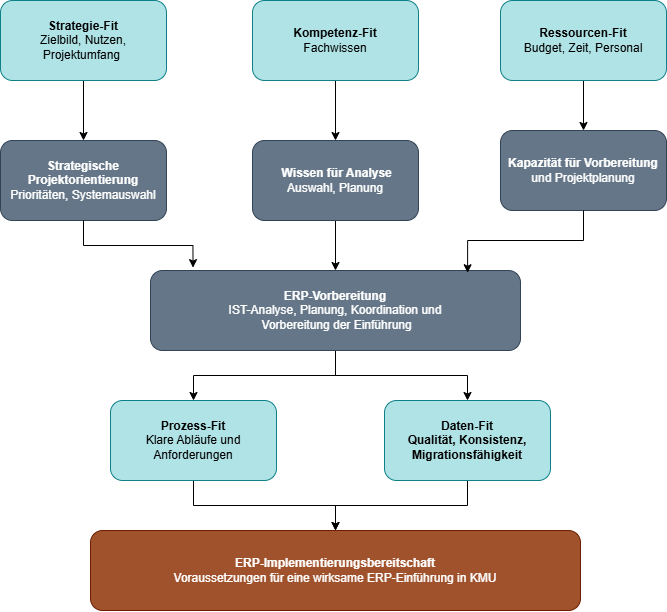
\includegraphics[
    width=\textwidth,
    keepaspectratio
  ]{figures/erp-kmu-fit-modell.png}
  \caption{Wirklogik des ERP-KMU-Fit-Modells, eigene Darstellung auf Basis
  der ausgewerteten Literatur}
  \label{fig:erp-kmu-fit-modell}
\end{figure}

ERP-Implementierungsbereitschaft liegt vor, wenn alle fünf Fit-Dimensionen in
einem ausreichenden Mindestmaß erfüllt sind. Defizite in einer Dimension können
dabei die Vorbereitung in anderen Bereichen beeinträchtigen. Fehlende
Ressourcen können beispielsweise die Prozessanalyse oder Datenbereinigung
erschweren, während fehlendes Wissen eine unpassende Systemauswahl oder eine
unzureichende Projektplanung begünstigen kann.

